\chapter{Infinite Sequences and Series}

\section{Sequences}
A \textbf{sequence} can be thought of as a list of numbers in definite order:
$$ a_1, a_2, a_3, a_4, \dots, a_n,\dots $$
which can also be denoted by
$$ \{a_n\} \qquad or \qquad \{a_n\}_{n=1}^\infty $$

\subsection*{Definition}
A sequence $\{a_n\}$ has the \textbf{limit} $L$ and we write
$$ \lim_{n \to \infty}a_n = L \qquad or \qquad a_n \rightarrow L \quad as \quad n \rightarrow \inf $$
if $\lim_{n \to \infty}a_n$ exists, we say the sequence \textbf{converges}).
Otherwise, we say the sequence \textbf{diverges}.

\subsection*{Definition}
A sequence $\{a_n\}$ has the \textbf{limit} $L$ and we write
$$ \lim_{n \to \infty}a_n = L \qquad or \qquad a_n \rightarrow L \quad as \quad n \rightarrow \inf $$
if for every $\epsilon >$ 0 there is corresponding integer $N$ such that
$$ if \quad n>N \quad then \quad |a_n - L|<\epsilon $$

\subsection*{Theorem}
if $\lim_{x \to \infty}f(x)=L$ and $f(n)=a_n$ when $n$ is an integer,
then $\lim_{n \to \infty}a_n=L$

\subsection*{Definition}
$\lim_{n \to \infty}a_n=\infty$ means that for every positive number $M$
there is an integer $N$ such that
$$ if \quad n>N \quad then \quad a_n>M $$

\subsection*{Theorem}
If $\lim_{n \to \infty}|a_n|=0$, then $\lim_{a \to \infty}a_n=0$

\subsection*{Theorem}
If $\lim_{n \to \infty}a_n=L$ and the function $f$ is continuous at $L$, then
$$ \lim_{n \to \infty}f(a_n) = f(L) $$

A sequence \{$r^n$\} is convergent if $-1<r\leq1$ and divergent for all other values of $r$.
$$ \lim_{n \to \infty}r^n =
    \begin{cases}
        0 & \text{if $-1<r\leq1$} \\
        1 & \text{if $r=1$}
    \end{cases} $$

\subsection*{Example}
Find $\lim_{n\to \infty}sin(\pi /n)$.

\subsection*{Solution}
Because the sine function is continuous at 0,
$$\lim_{n\to \infty}sin(\pi /n)=sin\left(\lim_{n\to \infty}(\pi /n)\right)=sin\:0=0$$

\subsection*{Definition}
A sequence \{$a_n$\} is called \textbf{increasing} if $a_n < a_{n+1}$
for all $n \geq 1$, that is $a_1<a_2<a_3<\dots$. It is called \textbf{decreasing}
if $a_n>a_{n+1}$ for all $n \geq 1$. A sequence is \textbf{monotonic}
if it's either increasing or decreasing.

\subsection*{Example}
Show that the sequence $a_n-\cfrac{n}{n^2+1}$ is decreasing.

\subsection*{Solution}
Consider the function $f(x)=\cfrac{x}{x^2+1}$:
$$f'(x)=\frac{x^2+1-2x^2}{(x^2+1)^2}=\frac{1-x^2}{(x^2+1)^2}<0$$
Thus $f$ is decreasing on $(1,\infty)$ and so $f(n)>f(n+1)$. Therefore ${a_n}$ is decreasing.

\subsection*{Definition}
A sequence \{$a_n$\} is \textbf{bounded above} if there is a number $M$ such that
$$ a_n \leq M \qquad for all n \geq 1 $$
It is \textbf{bounded below} if there is a number $m$ such that
$$ m \leq a_n \qquad for all n \geq 1 $$
It is bounded above and below, then \{$a_n$\} is a \textbf{bounded sequence}

\subsection*{Monotonic Sequence Theorem}
Every bounded, monotonic sequence is convergent.

\section{Series}
If we try to add the terms if an infinite sequence $\{a_n\}_{n=1}^\infty$
we get an expression of the form
$$ a_1+a_2+a_3+\dots+a_n+\dots $$
which is an \textbf{infinite series} (or just a \textbf{series}) and is denoted by
$$ \sum_{n=1}^{\infty} a_n \qquad or \qquad \sum a_n $$

\subsection*{Definition}
Given a series $\sum_{n=1}^n a_n = a_1+a_2+a_3+\dots$, let $s_n$ denote
its $n$th partial sum:
$$ s_n=\sum_{i=1}^n a_i = a_1+a_2+\dots + a_n $$
If the sequence \{$s_n$\} is convergent and $\lim_{n \to \infty} s_n =s$
exists as a real number, then the series $\sum a_n$ is called
\textbf{convergent} and we write
$$ a_1 + a_2 + \dots + a_n + \dots = s \qquad or \qquad \sum_{n=1}^\infty a_n = s$$
The number $s$ is called the \textbf{sum} of the series. If the sequence
\{$s_n$\} is divergent, then the series is called \textbf{divergent}. \par\null\par
\noindent The geometric series
$$ \sum_{n=1}^\infty ar^{n-1} = a + ar + ar^2 + \dots $$
is convergent if $|r| < 1$ and its sum is
$$ \sum_{n=1}^\infty ar^{n-1}=\frac{a}{1-r} \qquad |r|<1 $$
If $|r| \geq 1$, the geometric series is divergent.

\subsection*{Example}
Is the series $\sum_{n=1}^\infty 2^{2n}3^{1-n}$ convergent or divergent?

\subsection*{Solution}
Let's rewrite the $n$th term of the series in the form $ar^{n-1}$:
$$\sum_{n=1}^\infty 2^{2n}3^{1-n}=\sum_{n=1}^\infty (2^2)^n3^{-(n-1)}=
    \sum_{n=1}^\infty\frac{4^n}{3^{n-1}}=\sum_{n=1}^\infty 4\left(\frac{4}{3}\right)^{n-1}$$
This is a geometric series with $a=4$ and $r=\frac{4}{3}$. Since $r>1$, the series
diverges by (4).

\subsection*{Theorem}
If the series $\sum_{n=1}^\infty a_n$ is convergent, then
$\lim_{n \to \infty} a_n = 0$.

\subsection*{Test for Divergence}
If $\lim_{n \to \infty} a_n$ does not exist or if $\lim_{n \to \infty} a_n \neq 0$,
then the series $\sum_{n=1}^\infty a_n$ is divergent.

\subsection*{Example}
Show that the series $\sum_{n=1}^\infty \frac{n^2}{5n^2+4}$ diverges.

\subsection*{Solution}
$$\lim_{n\to \infty}a_n=lim_{n\to \infty}\frac{n^2}{5n^2+4}=
    lim_{n\to \infty}\frac{1}{5+4/n^2}=\frac{1}{5}\neq0$$
So the series diverges by the Test for Divergence.

\subsection*{Theorem}
If $\sum a_n$ and $\sum b_n$ are convergent series, then so are the series
$\sum ca_n$ (where $c$ is constant), $\sum (a_n+b_n)$, and $\sum(a_n-b_n)$, and
\begin{enumerate}[(i)]
    \item $\sum_{n=1}^\infty ca_n = c\sum_{n=1}^\infty a_n$
    \item $\sum_{n=1}^\infty(a_n+b_n)=\sum_{n=1}^\infty a_n + \sum_{n=1}^\infty b_n$
    \item $\sum_{n=1}^\infty(a_n-b_n)=\sum_{n=1}^\infty a_n - \sum_{n=1}^\infty b_n$
\end{enumerate}

\section{The Integral Test and Estimates of Sums}

\subsection*{The Integral Test}
Suppose $f$ is a continuous, positive, decreasing, function on $[1, \infty)$ and let
$a_n = f(n)$. Then the series $\sum_{n=1}^\infty a_n$ is convergent if and only if
the improper integeral $\int_1^\infty f(x) dx$ is convergent. In other words:
\begin{enumerate}[(i)]
    \item If $\int_1^\infty f(x) dx$ is convergent, then $\sum_{n=1}^\infty a_n$ is convergent.
    \item If $\int_1^\infty f(x) dx$ is divergent, then $\sum_{n=1}^\infty a_n$ is divergent.
\end{enumerate}
The $p$-series $\sum_{n=1}^\infty \frac{1}{n^p}$ is convergent if $p>1$ and divergent if $p \leq 1$.

\subsection*{Example}
Test the series $\sum_{n=1}^\infty\frac{1}{n^2+1}$ for convergence or divergence.

\subsection*{Solution}
The function $f(x)=1/(x^2+1)$ is continuous, positive, and decreasing on $[1,\infty)$
so we use the Integral Test:
$$\int_1^\infty \frac{1}{x^2+1}dx=\lim_{t\to\infty}\int_1^t\frac{1}{x^2+1}dx=
    \lim_{t\to\infty}tan^{-1}x]_1^t$$
$$=\lim_{t\to\infty}\left(tan^{-1}t-\frac{\pi}{4}\right)=\frac{\pi}{2}-\frac{\pi}{4}=\frac{\pi}{4}$$
The integral converges and so the series is convergent/

\section{The Comparison Tests}

\subsection*{The Comparison Test}
Suppose that $\sum a_n$ and $\sum b_n$ are series with positive terms.
\begin{enumerate}[(i)]
    \item If $\sum b_n$ is convergent and $a_n \leq b_n$ for all $n$, then $\sum a_n$ is also convergent.
    \item If $\sum b_n$ is divergent and $a_n \geq b_n$ for all $n$, then $\sum a_n$ is also divergent.
\end{enumerate}

\subsection*{Example}
Determine whether the series $\sum_{n=1}^\infty\frac{5}{2n^2+4n+3}$ converges or diverges.

\subsection*{Solution}
$$\frac{5}{2n^2+4n+3} < \frac{5}{2n^2}$$
We know that
$$\sum_{n=1}^\infty\frac{5}{2n^2}=\frac{5}{2}\sum_{n=1}^\infty\frac{1}{n^2}$$
is convergent because it's a $p$-series with $p=2>1$. Therefore
$$\sum_{n=1}^\infty\frac{5}{2n^2+4n+3}$$
is convergent by part (i) of the Comparison Test

\subsection*{The Limit Comparison Test}
Suppose that $\sum a_n$ and $\sum b_n$ are series with positive terms. If
$$ \lim_{n \to \infty} \frac{a_n}{b_n} = c $$
where $c$ is a finite number and $c>0$, then either both series converge or diverge.

\subsection*{Example}
Test the series $\sum_{n=1}^\infty\frac{1}{2^n-1}$ for convergence or divergence.

\subsection*{Solution}
We use the Limit Comparison Test with
$$a_n=\frac{1}{2^n-1} \qquad b_n=\frac{1}{2^n}$$
and obtain
$$\lim_{n\to\infty}\frac{a_n}{b_n}=\lim_{n\to\infty}\frac{1/(2^n-1)}{1/2^n}=
    \lim_{n\to\infty}\frac{2^n}{2^n-1}=\lim_{n\to\infty}\frac{1}{1-1/2^n}=1>0$$
Since this limit exists and $\sum 1/2^n$ is a convergent geometric series, the given
converges by the Limit Comparison Test.

\section{Alternating Series}
An \textbf{alternating series} is a series whose terms are alternately positive and negative.
$$ 1-\frac{1}{2}+\frac{1}{3}-\frac{1}{4}+\frac{1}{5}-\frac{1}{6}+\dots = \sum_{n=1}^\infty (-1)^{n-1} \frac{1}{n} $$

\subsection*{Alternating Series Test}
If the alternating series
$$ \sum_{n=1}^\infty(-1)^{n-1}b_n=b_1-b_2+b_3-b_4+b_5-b_6+\dots \quad b_n>0 $$
satisfies
\begin{enumerate}[(i)]
    \item $b_{n+1} \leq b_n \qquad$ for all $n$
    \item $lim_{n \to \infty} b_n = 0$
\end{enumerate}
then the series is convergent.

\subsection*{Example}
The alternating harmonic series
$$1-\frac{1}{2}+\frac{1}{3}-\frac{1}{4}+\dots = \sum_{n=1}^\infty\frac{(-1)^{n-1}}{n}$$
satisfies
\begin{enumerate}[(i)]
    \item $b_{n+1}<b_n \quad$ because $\quad \frac{1}{n+1}<\frac{1}{n}$
    \item $\lim_{n\to\infty}b_n=\lim_{n\to\infty}\frac{1}{n}=0$
\end{enumerate}
so the series is convergent by the Alternating Series Test.

\subsection*{Alternating Series Estimation Theorem}
If $s= \sum (-1)^{n-1}b_n$, where $b_n>0$, is the sum of an alternating series that satisfies
$$ (i)\: b_{n+1} \leq b_n \qquad and \qquad (ii)\: \lim_{n \to \infty} b_n = 0 $$
then
$$ |R_n|=|s-s_n| \leq b_{n+1}$$

\section{Absolute Convergence and the Ratio and Root Tests}

\subsection*{Definition}
A series $\sum a_n$ is called \textbf{absolutely convergent} if the series of absolute
values $\sum |a_n|$ is convergent.

\subsection*{Definition}
A series $\sum a_n$ is called \textbf{conditionally convergent} if it is convergent but
not absolutely convergent.

\subsection*{Theorem}
If a series $\sum a_n$ is absolutely convergent, then it is convergent.

\subsection*{The Ratio Test}
\begin{enumerate}[(i)]
    \item If $\lim_{n \to \infty} |\frac{a_{n+1}}{a_n}| = L < 1$, then the series
          $\sum_{n=1}^\infty a_n$ is absolutely convergent
    \item If $\lim_{n \to \infty} |\frac{a_{n+1}}{a_n}| = L > 1$ or
          $\lim_{n \to \infty} |\frac{a_{n+1}}{a_n}| = \infty$, then the series $\sum_{n=1}^\infty a_n$ is divergent.
          \enlargethispage{\baselineskip}
    \item If $\lim_{n \to \infty} |\frac{a_{n+1}}{a_n}| = 1$, the Ratio Test is inconclusive; that is,
          no conclusion can be drawn about the convergence or divergence of $\sum a_n$
\end{enumerate}

\subsection*{Example}
Test the convergence fo the series $\sum_{n=1}^\infty\frac{n^n}{n!}$.

\subsection*{Solution}
Since the terms $a_n=n^n/n!$ are positive, we don't need the absolute value signs.
$$\frac{a_{n+1}}{a_n}=\frac{(n+1)^{n+1}}{(n+1)!}\cdot\frac{n!}{n^n}=
    \frac{(n+1)(n+1)^n}{(n+1)n!}\cdot\frac{n!}{n^n}$$
$$=\left(\frac{n+1}{n}\right)^n=\left(1+\frac{1}{n}\right)^n\to e$$
Since $e>1$, the given series divergent by the Ratio Test.

\subsection*{The Root Test}
\begin{enumerate}[(i)]
    \item If $\lim_{n \to \infty} \sqrt[n]{|a_n|} = L < 1$, then the series $\sum_{n=1}^\infty a_n$ is absolutely convergent
    \item If $\lim_{n \to \infty} \sqrt[n]{|a_n|} = L > 1$ or
          $\lim_{n \to \infty} \sqrt[n]{|a_n|} = \infty$, then the series $\sum_{n=1}^\infty a_n$ is divergent
    \item If $\lim_{n \to \infty} \sqrt[n]{|a_n|} = 1$, the Root Test is inconclusive.
\end{enumerate}

\subsection*{Example}
Test the convergence of the series $\sum_{n=1}^\infty(\frac{2n+3}{3n+2})^n$.

\subsection*{Solution}
$$a_n=\left(\frac{2n+3}{3n+2}\right)^n$$
$$\sqrt[n]{|a_n|}=\frac{2n+3}{3n+2}=\frac{2+\frac{3}{n}}{3+\frac{2}{n}}\to\frac{2}{3}<1$$
Thus the given series is absolutely convergent by the Root Test.

\section{Strategy for Testing Series}

\begin{enumerate}
    \item If the series is of the form $\sum \frac{1}{n^p}$, it is a $p$-series, which we know to be
          convergent if $p>1$ and divergent if $p<1$.
    \item If the series has the form $\sum ar^{n-1}$ or $\sum ar^n$, it is a geometric series, which
          converges if $|r|<1$ and diverges if $|r| \geq 1$. Some preliminary algebraic manipulation may be required to bring the series into this form.
    \item If the series has a form that is similar to a $p$-series or a geometric series, then one of
          the comparison tests should be considered. In particular, if an is a rational function or an algebraic function of $n$, then the series should be compared with a $p$-series. The comparison tests apply only to series with positive terms, but if $\sum a_n$ some negative terms, then we can apply the Comparison Test to $\sum |a_n|$ and test for absolute convergence.
    \item If you can see at a glance that $\lim_{n \to \infty} a_n \neq 0$, then the Test for Divergence should be used.
    \item If the series is of the form $\sum (-1)^{n-1} b_n$ or $\sum (-1)^n b_n$, then
          the Alternating Series Test is an obvious possibility.
    \item Series that involve factorials or other products are often conveniently tested using the Ratio Test.
          This test should not be used because $|\frac{a_{n+1}}{a_n}| \to 1$ as $n \to \infty$ for all $p$-series.
    \item If $a_n$ is of the form $(b_n)^n$, then the Root Test may be useful.
    \item If $a_n = f(n)$, where $\int_1^\infty f(x) dx$ is easily evaluated, then the Integral Test is effective.
\end{enumerate}

\section{Power Series}

A \textbf{power series} is a series of the form
$$ \sum_{n=0}^\infty c_nx^n = c_0+c_1x+c_2x^2+c_3x^3+\dots $$
where $x$ is the variable and the $c_n$'s are constants called the \textbf{coefficients}.

More generally, a series of the form
$$ \sum_{n=0}^\infty c_n(x-a)^n = c_0+c_1(x-a)+c_2(x-a)^2+\dots$$
is called a \textbf{power series in (x-a)} or a \textbf{power series centered at $a$}.

\subsection*{Example}
For what values of $x$ is the series $\sum_{n=0}^\infty n!x^n$ convergent?

\subsection*{Solution}
We use the Ratio Test. If we let $a_n$ denote the $n$the term of the series,
then $a_n=n!x^n$. If $x \neq 0$, we have
$$ \lim_{n \to \infty}\left|\frac{a_{n+1}}{a_n}\right|=\lim_{n \to \infty}
    \left|\frac{(n+1)!x^{n+1}}{n!x^n}\right|=\lim_{n \to \infty}(n+1)|x|=\infty $$
By the Ratio Test, the series diverges when $x \neq 0$. Thus the given series converges
only when $x=0$.

\subsection*{Theorem}
For a given power series $\sum_{n=0}^\infty c_n(x-a)^n$, there are only three possibilities:
\begin{enumerate}[(i)]
    \item The series converges only when $x=a$.
    \item The series converges for all $x$.
    \item There is a positive number $R$ such that the series converges if $|x-a|<R$
          and diverges if $|x-a|>R$
\end{enumerate}

The number $R$ in case (iii) is called the \textbf{radius of convergence} of the power
series. By convention, the radius of convergence is $R=0$ in case (i) and $R=\infty$
in case (ii). The \textbf{interval of convergence} in case (i) is a single point $a$.
In case (ii) the interval is $(-\infty,\infty)$. In case (iii) there are four possibilities
$$(a-R,a+R) \quad (a-R,a+R] \quad[a-R,a+R) \quad [a-R,a+R]$$

\section{Representations of Functions as Power Series}

We start with a familiar equation:
$$ \frac{1}{1-x}=1+x+x^2+x^3+\dots=\sum_{n=0}^\infty x^n \qquad |x|<1 $$

\subsection*{Example}
Find a power series representation for 1/(x+2)

\subsection*{Solution}
In order to put this equation in the proper form, we factor a 2 from the denominator:
$$ \frac{1}{2+x}=\frac{1}{2(1+\frac{x}{2})}=\frac{1}{2[1-(-\frac{x}{2})]}=
    \frac{1}{2}\sum_{n=0}^\infty\left(-\frac{x}{2}\right)^n=\sum_{n=0}^\infty\frac{(-1)^n}{2^{n+1}}x^n$$
The series converges when $|\frac{-x}{2}|<1$, or $|x|<2$. So the interval of convergence is $(-2,2)$.

\subsection*{Term-by-Term Differentiation and Integration}
If the power series $\sum c_n(x-a)^n$ has a radius of convergence $R>0$,
then the function $f$ defined by
$$ f(x)=c_0+c_1(x-a)+c_2(x-a)^2+\dots=\sum_{n=0}^\infty c_n(x-a)^n $$
is differentiable and continuous on the interval $(a-R,a+R)$ and
\begin{enumerate}[(i)]
    \item $f'(x)=c_1+2c_2(x-a)+3c_3(x-a^2)+\dots=\sum_{n=1}^\infty nc_n(x-a)^{n-1}$
    \item $\int f(x)dx=C+c_0(x-a)+c_1\frac{(x-a)^2}{2}+c_2\frac{(x-a)^3}{3}+\dots=C+
              \sum_{n=0}^\infty c_n \frac{(x-a)^{n+1}}{n+1}$
\end{enumerate}
The radii of convergence of the power series in both Equations is $R$.

\section{Taylor and Maclaurin Series}

\subsection*{Theorem}
If $f$ has a power series expansion at $a$, which is
$$ f(x)=\sum_{n=0}^\infty c_n(x-a)^n \qquad |x-a|<R $$
then its coefficients are given by the formula
$$ c_n=\frac{f^{(n)}(a)}{n!} $$

Substituting the formula for $c_n$ into the series $f$ must be of the following form
$$ f(x)=\sum_{n=0}^\infty \frac{f^{(n)}(a)}{n!} (x-a)^n=f(a)+\frac{f'(a)}{1!}(x-a)+\frac{f''(a)}{2!}(x-a)^2+\dots $$
This series is called the \textbf{Taylor series of the function $f$ about $a$}
For the special case $a=0$ the Taylor series becomes
$$ f(x)=\sum_{n=0}^\infty \frac{f^{(n)}(0)}{n!}x^n=f(0)+\frac{f'(0)}{1!}x+\frac{f''(0)}{2!}x^2+\dots $$

\subsection*{Theorem}
If $f(x)=T_n(x)+R_n(x)$, where $T_n$ is the $n$th-degree Taylor polynomial of $f$ at $a$ and
$$ \lim_{n \to \infty} R_n(x)=0 $$
for $|x-a|<R$, then $f$ is equal to the sum of its Taylor series on the interval $|x-a|<R$.

\subsection*{Example}
Find the Maclaurin series for sin $x$ and prove that it represents sin $x$ for all $x$.

\subsection*{Solution}
We arrange our computation in two columns:
\begin{center}
    $\begin{array}{ll}
            f(x)=sinx  & f(0)=0     \\
            f(x)=cosx  & f'(0)=1    \\
            f(x)=-sinx & f''(0)=0   \\
            f(x)=-cosx & f'''(0)=-1 \\
            f(x)=sinx  & f^{4}(0)=0
        \end{array}$
\end{center}

Since the derivatives repeat in a cycle of four, we write the Maclaurin as follows:
$$ f(0)+\frac{f'(0)}{1!}x+\frac{f''(0)}{2!}x^2+\frac{f'''(0)}{3!}x^3+\dots$$
$$=x-\frac{x^3}{3!}+\frac{x^5}{5!}-\frac{7^3}{7!}+\dots=\sum_{n=0}^\infty(-1)^n\frac{x^{2n+1}}{(2n+1)!} $$
\pagebreak

\textbf{Important Maclaurin Series and Their Radii of Convergence}
\begin{center}
    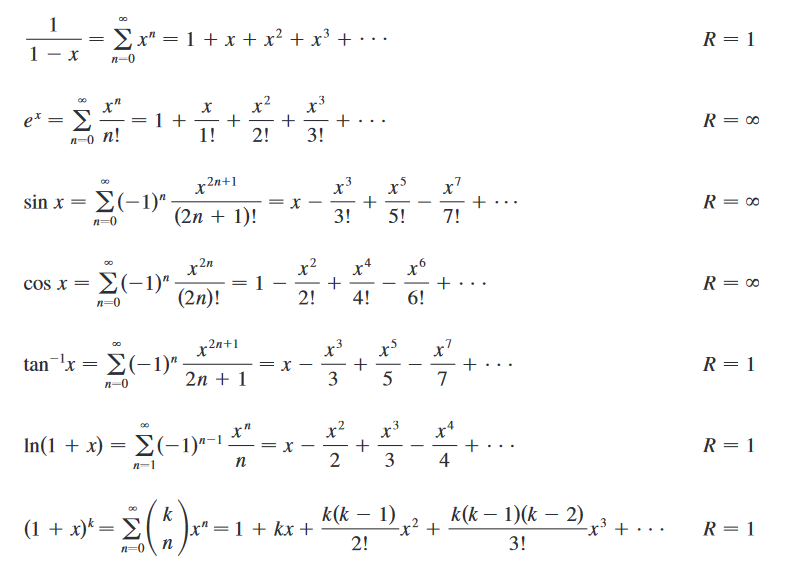
\includegraphics[scale=0.7]{table12-10}
\end{center}

\section{Applications of Taylor Polynomials}

\subsection*{Approximating Functions by Polynomails}

\subsection*{Example}
\begin{enumerate}[(a)]
    \item Approximate the function $f(x)=\sqrt[3]{x}$ by a Taylor
          polynomial of degree 2 at $a=8$.
    \item How accurate is this approximation when $7\leq x \leq 9$?
\end{enumerate}

\subsection*{Solution}
(a)
\begin{center}
    $\begin{array}{ll}
            f(x)=x^{1/3}                & f(8)=2               \\
            f'(x)=\frac{1}{3}x^{-2/3}   & f'(8)=\frac{1}{12}   \\
            f''(x)=-\frac{2}{9}x^{-5/3} & f''(8)=\frac{1}{144} \\
            f'''(x)=\frac{10}{27}x^{-8/3}
        \end{array}$
\end{center}
Using the second-degree Taylor polynomial, $T_2(x)$, the desired approximation is
$$ \sqrt[3]{x} \approx T_2(x) = 2+\frac{1}{12}(x-8)-\frac{1}{288}(x-8)^2 $$
(b) The tailor series is not alternating when $x<8$, so we can't use the Alternating
Series Estimation Theorem. But we can use the Taylor's Inequality with $n=2$ and $a=8$:
$$ |R_2(x)| \leq \frac{M}{3!}|x-8|^3 $$
where $|f'''(x)|\leq M$. Because $x \geq 7$, we have $x^{8/3} \geq 7^{8/3}$ and so
$$ f'''(x)=\frac{10}{27} \cdot \frac{1}{x^{8/3}} \leq \frac{10}{27} \cdot \frac{1}{7^{8/3}}<0.0021$$
Thereform we can take $M=0.0021$. Also $7\leq x\leq 9$, so $-1\leq x-8\leq 1$ and
$|x-8|\leq 1$. Then Taylor's Inequality gives
$$ |R_2(x)| \leq \frac{0.0021}{3!} \cdot 1^3=\frac{0.0021}{6} < 0.0004 $$
Thus, if $7\leq x\leq 9$, the approximation in part (a) is accurate within 0.0004.